\chapter[{Local gauge invariance and the form of interaction}]{Local gauge invariance and determination of the form of interaction}
\chaptermark{Local gauge invariance}

\section{Local gauge invariance of the electromagnetic field}

The Dirac equation is required to be covariant (of the same form) if the wavefunction undergoes a local phase transformation:

\[
  \psi \to \psi' = \e^{iq\alpha(\ul{r})}\psi
\]

Note that $\alpha$, the phase, is a function of the coordinates and not a simple constant.

The Dirac equation is:

\[
  \left(i\gamma_{\mu}\partial^{\mu} - q\gamma_{\mu}A^{\mu} - m\right) = 0
\]

Under a local gauge transformation:

\begin{eqnarray*}
  \left(i\gamma_{\mu}\partial^{\mu} - q\gamma_{\mu}A'^{\mu} - m\right)\e^{iq\alpha(\ul{r})}\psi & = & 0 \\
  \Rightarrow \e^{iq\alpha(\ul{r})}\left(i\gamma_{\mu}\partial^{\mu} + i \gamma_{\mu}iq\partial^{\mu}\alpha - q\gamma_{\mu}A'^{\mu} - m\right)\psi & = & 0 \\
  \textrm{But } A'^{\mu} & = & A^{\mu} - \partial^{\alpha} \\
  \Rightarrow \e^{iq\alpha(\ul{r})}\left(i\gamma_{\mu}\partial^{\mu} - \gamma_{\mu}q\partial^{\mu}\alpha - q\gamma_{\mu}A^{\mu} + q\gamma_{\mu}\partial^{\mu}\alpha - m\right) & = & 0
\end{eqnarray*}

If the Dirac equation is required to be covariant under local gauge transformations then the massless electromagnetic field must be introduced where $A^{\mu}$ is invariant under the gauge transformation $A'^{\mu} = A^{\mu} - \partial^{\mu}\alpha(\ul{r})$.  This involves replacing $i\partial^{\mu}$ in the Dirac equation by $\partial^{\mu} - qA^{\mu}$ or $\partial^{\mu}$ by $\partial^{\mu} + iqA^{\mu} = D^{\mu}$.  So it is necessary to demonstrate that$D^{\mu}\psi$ transforms the same was as $\psi$.  ie:

\[
  \left(D^{\mu}\psi\right)' = \e^{iq\alpha(\ul{r})}D^{\mu}\psi
\]

\begin{eqnarray*}
  \left( D^{\mu}\psi\right)' & = & \left(\partial^{\mu} + iqA'^{\mu}\right)\e^{iq\alpha(\ul{r})}\psi \\
  & = & \e^{iq\alpha(\ul{r})}\left( \partial^{\mu} + iq\partial^{\mu}\alpha + iqA^{\mu} - iq\partial^{\mu}\alpha\right)\psi \\
  & = & \e^{iq\alpha(\ul{r})}\left(\partial^{\mu} + iqA^{\mu}\right)\psi \\
   & = & \e^{iq\alpha(\ul{r})}D^{\mu}\psi
\end{eqnarray*}

Consider the Lagrangian field theory formalism.  For the free Dirac equations, a Lagrangian can be constructed such that a simple operation yields the Dirac equation.

\[
  L = i\bar{\psi}\gamma_{\mu}\partial^{\mu}\psi - m\bar{\psi}\psi
\]

Applying the Euler-Lagrange equation yields:

\[
  \left(i\gamma_{\mu}\partial^{\mu} - m\right)\psi = 0
\]

There is also a Lagrangian for the Klein-Gordon equation:

\[
  L = \frac{1}{2}\partial_{\mu}\phi\partial^{\mu}\phi - \frac{1}{2}m^2\phi^2
\]

Introducing the massless field modifies the Lagrangian to:

\begin{eqnarray*}
  L & = & i\bar{\psi}\gamma_{\mu}D^{\mu}\psi - m\bar{\psi}\psi \\
    & = & \bar{\psi}\left(i\gamma_{\mu}\partial^{\mu} - m\right)\psi - q\bar{\psi}\gamma_{\mu}\psi A^{\mu}
\end{eqnarray*}

Hence, by demanding local gauge invariance it is necessary to introduce a vector field.  $A_{\mu}$ is called the gauge field, which couples to the Dirac particle (charge $q$) in exactly  the same way as the photon field.  Indeed the new interaction term may be written as $-j_{\mu}A^{\mu}$ where $j_{\mu} = -\e\bar{\psi}\gamma_{\mu}\psi$ is the current density.

If this new field is considered as a physical photon field then a term corresponding to its kinetic energy must be added.  As the kinematic term must be invariant it can only involve the gauge invariant field tensor.

\[
  F_{\mu\nu} = \partial_{\mu}A_{\nu} - \partial_{\nu}A_{\mu}
\]

So the Lagrangian of QED is:

\[
  L_{QED} = \bar{\psi}\left(i\gamma_{\mu}\partial^{\mu} - m\right)\psi + \e\bar{\psi}\gamma_{\mu}A^{\mu}\psi - \frac{1}{4}F_{\mu\nu}F^{\mu\nu}
\]

The addition of a mass term is prohibited by gauge invariance.  Substitute $A'^{\mu} \to A^{\mu} + \partial^{\mu}\alpha$ into the Proca equation and it changes; only when $m=0$ does the Proca equation remain the same.  Therefore the photon must be massless.  The photon couples only to charged particles and therefore has no self-coupling.

\section{Local gauge invariance and the electroweak interaction}

The electroweak interaction acts between left-handed doublet weak isospinors $\chi_L$ and right-handed weak isospin singlets $\chi_R$.  Hypercharge is the "charge like" object in weak isospin space.

The left-handed and right-handed components transform as:

\begin{eqnarray*}
  \chi_L & \to \chi'_L & = \e^{ig_W\alpha(\ul{r})\frac{\tau}{2} + i\frac{g'}{2}\beta(x)Y}\chi_L \\
  \chi_R & \to \chi'_R & = \e^{i\frac{g'}{2}\beta(\ul{r})Y}\chi_R
\end{eqnarray*}

For a Dirac-like equation to remain covariant under such a local gauge transformation four massless fields must be introduced: $W_{\mu}^1$, $W_{\mu}^2$, $W_{\mu}^3$ and $B_{\mu}$ in the following way:

\begin{eqnarray*}
  L = & \bar{\chi}_L\gamma^{\mu}\left(i\partial_{\mu} - \frac{g_W}{2}\tau W_{\mu} - \frac{g'}{2}YB_{\mu}\right)\chi_L & || SU(2) \\
  & + \bar{\psi}_R\gamma^{\mu}\left(i\partial_{\mu} - \frac{g'}{2}YB_{\mu}\right)\psi_R & || U(1)_Y \\
  & - \frac{1}{4}W_{\mu\nu}W^{\mu\nu} - \frac{1}{4}B_{\mu\nu}B^{\mu\nu}
\end{eqnarray*}

where the last two terms are the kinetic energy and self-coupling of the $W_{\mu}$ and $B_{\mu}$ fields.

Note that there is no mass term above.  Adding simple mass terms is not possible as they are not gauge invariant.  To add mass in a gauge invariant way, the Higgs mechanism in needed.

Mass terms are of the form:

\[
  \bar{\psi}m\psi = \left(\bar{\psi}_L + \bar{\psi}_R\right)m\left(\psi_L + \psi_R\right)
\]

Such terms would link a left-handed electron in the $SU(2)$ weak doublet to a right-handed electron, which is a singlet.  If $SU(2) \times U(1)$ symmetry were exact, this could not happen.  Also, for the fields introduced, $W_{\mu}^{1/2/3}$ and $B_{\mu}$, to preserve local gauge symmetry, they have to be massless since terms like $m^2B_{\mu}B^{\mu}$ do not preserve gauge invariance.

Consider how $W^{\mu}$ transforms under a gauge transformation:

\begin{eqnarray*}
  \chi'_L & = & \e^{ig_W\alpha(\ul{r})\frac{\tau}{2}}\chi_L \\
  \textrm{then } \left(D^{\mu}\chi_L\right)' & = & \e^{ig_W\alpha(\ul{r})\frac{\tau}{2}}D^{\mu}\chi_L
\end{eqnarray*}

For an infinitesimal change:

\begin{eqnarray*}
  W'_i{}^{\mu} & = & W_i^{\mu} + \delta W_i^{\mu} \\
  \textrm{LHS: } \left(D^{\mu}\chi_L\right)' & = & D'^{\mu}\chi'_L \\
  & = & \left(\partial^{\mu} + ig_W \frac{\tau_i}{2}W_i^{\mu} + ig_W\frac{\tau_i}{2}\delta W_i^{\mu}\right)\chi'_L \\
  \textrm{where } D^{\mu} & = & \partial^{\mu} + ig_W\frac{\tau}{2}W_i^{\mu} \\
  & = & \left(\partial^{\mu} + ig_W\frac{\tau_i}{2}W_i^{\mu} + ig_W\frac{\tau_i}{2}\delta W_i^{\mu}\right) \left(1 + ig_W\alpha(\ul{r})\frac{\tau_j}{2}\right)\chi_L \\
  & = & \left( \partial^{\mu} + ig_W\alpha\frac{\tau_j}{2}\partial^{\mu} + ig_W\frac{\tau_i}{2}W_i^{\mu} \right.\\
  & & \left.+ ig_W\partial^{\mu}\alpha\frac{\tau_j}{2} + ig_W ig_W \frac{\tau_i}{2}W_i^{\mu}\alpha\frac{\tau_j}{2} + ig_W\frac{\tau_i}{2}\delta W_i^{\mu}\right)\chi_L \\
  \textrm{RHS: } & = & \left(1 + ig_W\alpha\frac{\tau_j}{2}\right)\left(\partial^{\mu} + ig_W\frac{\tau_i}{2}W_i^{\mu}\right)\chi_L \\
  & = & \left(\partial^{\mu} + ig_W\frac{\tau_i}{2}W_i^{\mu} + ig_W\alpha\frac{\tau_j}{2}\partial^{\mu} \right.\\
  & & \left.+ ig_W\alpha\frac{\tau_j}{2}ig_W\frac{\tau_i}{2}W_i^{\mu}\right)\chi_L \\
  \textrm{LHS} & = & \textrm{RHS} \\
  ig_W\frac{\tau_i}{2}\delta W_i^{\mu} & = & ig_W\partial^{\mu}\alpha_j\frac{\tau_j}{2} - ig_Wig_W\frac{\tau_i}{2}\frac{\tau_j}{2}W_i^{\mu}\alpha + ig_Wig_W\frac{\tau_j}{2}\frac{\tau_i}{2}W_i^{\mu}\alpha_j \\
  \frac{\tau_i}{2}\delta W_i^{\mu} & = & -\frac{\tau_i}{2}\partial^{\mu}\alpha_i - ig_W\Bigg[\frac{\tau_i}{2},\frac{\tau_j}{2}\Bigg]\alpha_jW_i^{\mu} \\
  & = & -\frac{\tau_i}{2}\partial^{\mu}\alpha_i - ig_Wi\epsilon_{ijk}\frac{\tau_k}{2}\alpha_jW_i^{\mu} \\
  & = & -\frac{\tau}{2}\partial^{\mu}\alpha_i - g_W\frac{\tau_i}{2}\ul{\alpha}\times\ul{W} \\
  \Rightarrow \delta W_i^{\mu} & = & -\partial^{\mu}\alpha_i - g_W\ul{\alpha}\times\ul{W} \\
  \Rightarrow W_i^{\mu} \to W'_i{}^{\mu} & = & W_i^{\mu} - \partial^{\mu}\alpha_i - g_W \ul{\alpha}\times\ul{W}
\end{eqnarray*}

Now consider the self-interaction terms in the Lagrangian:

\begin{eqnarray*}
  -\frac{1}{4}W_{\mu\nu}W^{\mu\nu} & - & \frac{1}{4}B_{\mu\nu}B^{\mu\nu} \\
  \textrm{where } B_{\mu\nu}B^{\mu\nu} & = & \partial_{\mu}B^{\nu} - \partial^{\nu}B_{\mu}
\end{eqnarray*}

However, the $W_{\mu\nu}$ terms would not be invariant under gauge transformations if they were of this form.  Because of the extra term in $W'_i{}^{\mu}$, $W_{\mu\nu}$ has to be:

\[
  W_{\mu\nu} = \partial_{\mu}W_{\nu} - \partial_{\nu}W_{\mu} - g_W \ul{W}_{\mu}\times\ul{W}_{\nu}
\]

The $-\frac{1}{4}W_{\mu\nu}W^{\mu\nu}$ yields the trilinear and quadrilinear couplings of the weak bosons:

\begin{figure}[!htb]
  \begin{center}
    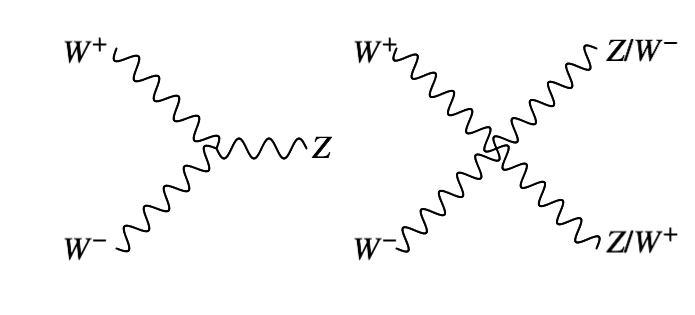
\includegraphics[width=\textwidth]{images/web_feynman/image_77.png}
    \caption[Trilinear and quadrilinear boson couplings]{Trilinear and quadrilinear boson couplings for $WW\to Z$ (left) and $WW\to WW$ (right).}
    \label{fig:ch15_vectorBosonScattering}
  \end{center}
\end{figure}

\begin{eqnarray*}
  -\frac{1}{4}W_{\mu\nu}W^{\mu\nu} & = & -\frac{1}{4} \Big[\partial^{\mu}W^{\nu} - \partial^{\nu}W^{\mu} - g_W W^{\mu}\times W^{\nu}\Big]\Big[\partial_{\mu}W_{\nu} - \partial_{\nu}W_{\mu} - g_W W_{\mu}\times W_{\nu}\Big] \\
  \textrm{Trilinear } & & -\frac{1}{4}\Big( \left(\partial^{\mu}W^{\nu} - \partial^{\nu}W^{\mu}\right)\left(\partial_{\mu}W_{\nu} - \partial_{\nu}W_{\mu}\right)\Big. \\
  \textrm{couplings: } & & -g_W\left(\partial^{\mu}W^{\nu} - \partial^{\nu}W^{\mu}\right)\left(W_{\mu}\times W_{\nu}\right) -g_W\left(W^{\mu}\times W^{\nu}\right)\left(\partial_{\mu}W_{\nu} - \partial_{\nu}W_{\mu}\right) \\
  \textrm{Quadrilinear } Big. & & + g_W^2\left(W^{\mu}\times W^{\nu}\right)\left(W_{\mu}\times W_{\nu}\right) \\
  \textrm{couplings: } & &
\end{eqnarray*}

\subsection{Trilinear coupling}

From the above, the $2^{nd}$ and $3^{rd}$ terms are the same.  Also:

\[
  \left(\partial_{\mu}W_{\nu} - \partial_{\nu}W_{\mu}\right)\left(W^{\mu}\times W^{\nu}\right) = 2\left(\partial_{\mu}W_{\nu}\right)\left(W^{\mu}\times W^{\nu}\right)
\]

So the trilinear coupling is:

\[
  -\frac{1}{4}4\left(\partial_{\mu}W_{\nu}\right)\left(W^{\mu}\times W^{\nu}\right)
\]

So at the vertex:

\begin{figure}[!htb]
  \begin{center}
    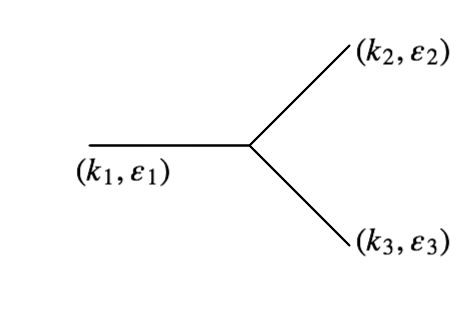
\includegraphics[width=0.5\textwidth]{images/web_feynman/image_78.png}
    \caption[Trilinear coupling variables]{Definitions of trilinear coupling variables, $(k_1,\varepsilon_1)$, $(k_2,\varepsilon_2)$, and $(k_3,\varepsilon_3)$.}
    \label{fig:ch15_trilinearVariables}
  \end{center}
\end{figure}

\begin{eqnarray*}
  W^1_{\nu} & = & \epsilon^1_{\nu}\e^{-ik^1_{\mu}x^{\mu}} \\
  \Rightarrow \partial_{\mu}W^1_{\nu} & = & -ik^1_{\mu}\epsilon^1_{\nu}\e^{-ik^1_{\mu}x^{\mu}} \\
  \textrm{So } -g_W\left(\partial_{\mu}W_{\nu}\right)W^{\mu}\times W^{\nu} & = & g_W
  \left|
  \begin{array}{ccc}
    ik^1_{\mu}\epsilon^1_{\nu} & ik^2_{\mu}\epsilon^2_{\nu} & ik^3_{\mu}\epsilon^3_{\nu} \\
    \epsilon_1^{\mu} & \epsilon_2^{\mu} & \epsilon_3^{\mu} \\
    \epsilon_1^{\nu} & \epsilon_2^{\nu} & \epsilon_3^{\nu}
  \end{array}
  \right|
  \\
  & = & ig_W \Big[ k^1_{\mu}\epsilon^1_{\nu}\left(\epsilon_2^{\mu}\epsilon_3^{\nu} - \epsilon_3^{\mu}\epsilon_2^{\nu}\right) - k^2_{\mu}\epsilon^2_{\nu}\left(\epsilon_1^{\mu}\epsilon_3^{\nu} - \epsilon_1^{\nu}\epsilon_3^{\mu}\right) + k^3_{\mu}\epsilon^3_{\nu}\left(\epsilon_1^{\mu}\epsilon_2^{\nu} - \epsilon_1^{\nu}\epsilon_2^{\mu}\right)\Big] \\
  & = & ig_W\Big[\left(\epsilon_1 \cdot \epsilon_2\right)\left(k_2 - k_1\right)\cdot \epsilon_3 + \left(\epsilon_2 \cdot \epsilon_3\right)\left(k_3 - k_2\right)\cdot \epsilon_1 + \left(\epsilon_3 \cdot \epsilon_1\right)\left(k_1 - k_3\right)\cdot \epsilon_3\Big]
\end{eqnarray*}

These are essentially the Feynmann rules for $3$ vectors at a vertex.

\subsection{Quadrilinear couplings}

The term for quadrilinear coupling is $\frac{1}{4}g_W^2\left(W_{\mu}\times W_{\nu}\right)\left(W^{\mu}\times W^{\nu}\right)$.  So these couplings will be the products of the four polarisation vectors ie $\left(\epsilon_1 \cdot \epsilon_2\right)\left(\epsilon_3 \cdot \epsilon_4\right)$.

\section{Local gauge invariance and QCD}

As with QED, the structure of QCD can be inferred from local gauge invariance.  Here $U(1)$ is replaced by $SU(3)$ group of phase transformations of colour fields.  Under local gauge transformations, the quark fields transform as:

\begin{eqnarray*}
  q(\ul{r}) \to q'(\ul{r}) & = & Uq(\ul{r}) \\
  \textrm{where } U & = & \e^{i\alpha_a(\ul{r})\frac{\lambda_a}{2}}
\end{eqnarray*}

and $\lambda_a$ are a set of linearly indepedent, traceless $3 \times 3$ matrices (Gell-Mann matrices) and $\alpha_a$ are the group parameters.  The $SU(3)$ generators do not commute, hence the theory is non Abelian:

\[
  \Bigg[\frac{\lambda_i}{2},\frac{\lambda_j}{2}\Bigg] = if_{ijk}\frac{\lambda_k}{2}
\]

Following the same formalism as for QED, $SU(3)$ invariance is imposed on the free Lagrangian.  Consider an infinitesimal transformation:

\begin{eqnarray*}
  q(\ul{r}) & \to & \left(1 + i\alpha_a(\ul{r})\frac{\lambda_a}{2}\right)q(ul{r}) \\
  \partial_{\mu}q & \to & \left(1 + i\alpha_a(\ul{r})\frac{\lambda_a}{2}\right)\partial_{\mu}q + i\frac{\lambda_a}{2}q\partial_{\mu}\alpha_a
\end{eqnarray*}

The eight gauge fields, $G^a_{\mu}$, are then introduced, which transform as:

\[
  G^a_{\mu} \to G^a_{\mu} - \frac{1}{g_s}\partial_{\mu}\alpha_a
\]

The covariant derivative is formed as:

\[
  D_{\mu} = \partial_{\mu} + ig_s\frac{\lambda_a}{2}G^a_{\mu}
\]

So the Lagrangian becomes:

\[
  L = \bar{q}\left(i\gamma^{\mu}\partial_{\mu} - m\right)q - g_s\bar{q}\gamma^{\mu}\frac{\lambda_{a}}{2}qG^a_{\mu}
\]

However this is not a gauge invariant Lagrangian.

\begin{eqnarray*}
 \textrm{So } \bar{q}\gamma^{\mu}\frac{\lambda_a}{2}q & \to & \bar{q}\gamma^{\mu}\frac{\lambda_a}{2}q + i\alpha_b\bar{q}\gamma^{\mu}\left(\frac{\lambda_a}{2}\frac{\lambda_b}{2} - \frac{\lambda_b}{2}\frac{\lambda_a}{2}\right)q \\
  & \to & \bar{q}\gamma^{\mu}\frac{\lambda_a}{2}q - f_{abc}\alpha_b\left(\bar{q}\gamma^{\mu}\frac{\lambda_c}{2}q\right)
\end{eqnarray*}

From this it can be seen that gauge invariance will be satisfied if the field transforms as:

\[
  G^a_{\mu} \to G^a_{\mu} - \frac{1}{g_s}\partial_{\mu}\alpha_a - f_{abc}\alpha_bG^c_{\mu}
\]

The kinetic energy is added (as before) for each of the fields and the QCD Lagrangian becomes:

\[
  L = \bar{q}\left(i\gamma^{\mu}\partial_{\mu} - m\right)q - g_s\left(\bar{q}\gamma^{\mu}\frac{\lambda_a}{2}q\right)G^a_{\mu} - \frac{1}{4}G^a_{\mu\nu}G_a^{\mu\nu}
\]

Writing alternatively:

%\[
%  L = \textrm{``}\bar{q}q\textrm{''} + \textrm{``}G\textrm{''}^2 + g_s\textrm{``}\bar{q}qG\textrm{''} + g_s\textrm{``}G\textrm{''}^3 + g_s^2\textrm{``}G\textrm{''}^4
%\]

\begin{figure}[!htb]
  \begin{center}
    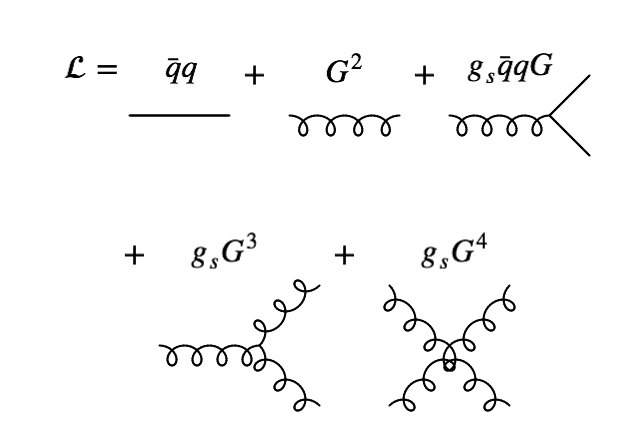
\includegraphics[width=\textwidth]{images/web_feynman/image_79.png}
    \caption[Multilinear QCD processes]{Multilinear QCD processes.}
    \label{fig:ch15_trilinearQuadrilinearQCD}
  \end{center}
\end{figure}

\section{Evolution of the coupling constants}

The self-coupling of gluons leads to a different behaviour of the QCD coupling constant $\alpha_s$, with $Q^2$ compared to the QED coupling.

\subsection{QED}

Loops can be introduced to processes which give rise to higher order terms in a calculation.

\begin{figure}[!htb]
  \begin{center}
    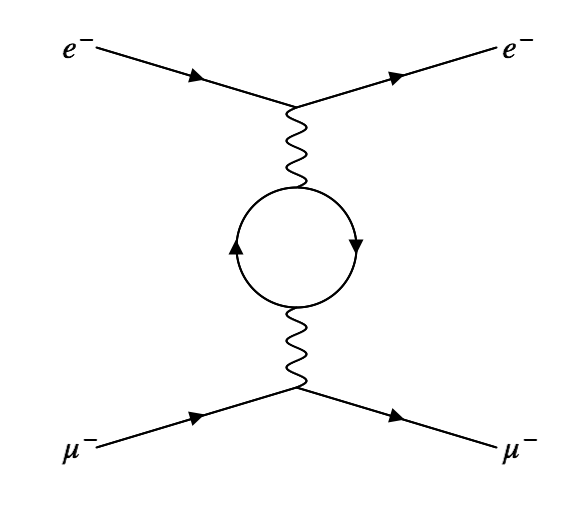
\includegraphics[width=0.5\textwidth]{images/web_feynman/image_80.png}
    \caption[Higher order QED process]{Higher order QED process.}
    \label{fig:ch15_higherOrderQED}
  \end{center}
\end{figure}

$\e \mu$ scattering with a virtual loop in the photon line adds the next order of calculations.  This diagram is calculable, but there is no restriction on the $4-$momentum of these loop particles and so the loops are infinite.

The electron charge (say) becomes dependent on the scale of the process and had to be renormalised to remove infinities present in the loop calculations.

\begin{figure}[!htb]
  \begin{center}
    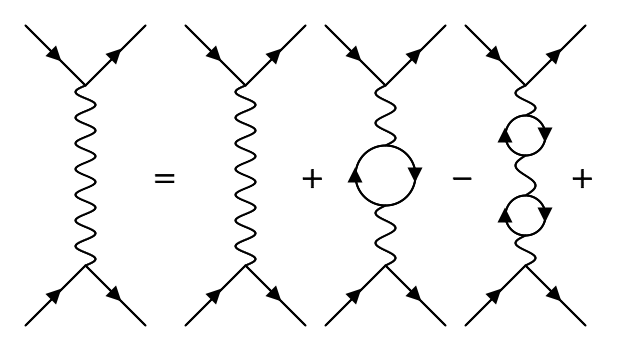
\includegraphics[width=\textwidth]{images/web_feynman/image_81.png}
    \caption[Many-loop QED process]{Many-loop QED process.}
    \label{fig:ch15_manyLoopQED}
  \end{center}
\end{figure}

and the relationship between the measured $\e^2$ and the ``bare'' $\e^2_0$ has to be specified at a particular $Q^2$.  As the coupling is directly related to the charge, this also then has a $Q^2$ dependence: the ``running coupling constant'', $\alpha(Q^2)$, given by:

\[
  \alpha(Q^2) = \frac{\alpha(\mu^2)}{1 - \frac{\alpha(\mu^2)}{3\pi}\ln\left(\frac{Q^2}{\mu^2}\right)}
\]

where $\mu$ is the renormalisation scale.

\subsection{QCD}

For QCD, all the couplings derived previously contribute, so:

\begin{figure}[!htb]
  \begin{center}
    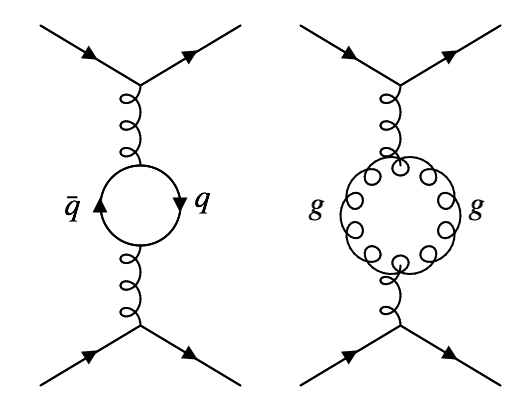
\includegraphics[width=0.75\textwidth]{images/web_feynman/image_82.png}
    \caption[Single loop QED and QCD processes]{Single loop QED and QCD processes.}
    \label{fig:ch15_loopQEDQCD}
  \end{center}
\end{figure}

\[
  \alpha_s(Q) = \frac{\alpha_s(\mu^2)}{1 + \frac{\alpha_s(\mu^2)}{12\pi}\left(33 - 2n_f\right)\ln\left(\frac{Q^2}{\mu^2}\right)}
\]

The coupling $\alpha_s(Q^2)$ decreases with increasing $Q^2$ and therefore becomes small for short-distance interaction, leading to asymptotic freedom.  Perturbation theory can also then be applied for high $Q^2$.
